\chapter{Introduction}\label{ch:intro}

Typical networking-focused systems face major problems with either security, performance or both.
This thesis explores a novel I/O framework on seL4 for secure, high-performance
networking-based systems and extends the framework to support multi-client systems.

\section{The problem with I/O on monolithic kernels}
Operating systems are designed to abstract over hardware while
providing a consistent interface to applications. In a monolithic kernel
such as Linux, the kernel houses device drivers, file systems and network 
stacks. This means that these services run in privileged mode, and user 
applications make system calls in order to utilise these services and perform I/O.
However, there are two major problems with this design:
it is inherently insecure and historically, performs poorly.

\subsection{Monolithic kernels are fundamentally insecure}
Modern operating systems see a rapid development rate on a huge code base.
\autoref{f:growth} shows the exponential growth of the Linux kernel
(extracted from \cite{Linux:archives}) which sees over 70 thousand commits a year.
With this growth, bugs and security vulnerabilities are steadily brought into the 
trusted computing base.

\begin{figure}[h]
  \centering
  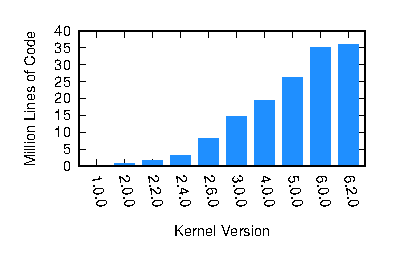
\includegraphics[width=10cm]{growth.eps}
  \caption{Growth of the Linux Kernel.}
  \label{f:growth}
\end{figure}

While much of this growth can be attributed to kernel extensions, such as drivers for new devices,
these extensions should not be overlooked. A modern Linux kernel runs around 80 - 130
device drivers on a given configuration \cite{Linux:LKDDB}, and drivers account for a significant
portion of critical vulnerabilities and exposures (CVE). \autoref{f:cves} shows the proportion of 
CVEs published in the last 5 years that can be attributed directly to drivers (extracted 
from \cite{Linux:CVEs}), with an average of 38\%.

\begin{figure}[h]
  \centering
  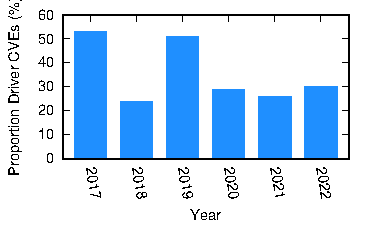
\includegraphics[width=10cm]{cves.pdf}
  \caption{Proportion of Linux CVEs due to device drivers.}
  \label{f:cves}
\end{figure}

The reason behind such a high rate of Linux CVEs is due largely to the fact that
drivers are typically written by hardware engineers as opposed to OS experts, and the growing
complexity of the kernel, has made kernel programming extremely difficult \cite{Swift_MLE_02}.\\
While modern kernels deploy a number of security mechanisms to protect their execution,
a large portion of vulnerabilities remains exploitable \cite{Narayanan_HTJB_20}. For example,
even advanced defence mechanisms, such as code pointer integrity (CPI) and safe stacks,
that protect the control flow of an application \cite{Kuznetsov_SPCSS_14}, remain
vulnerable to data-only attacks. These attacks, which focus on altering or forging
the critical data of an application can be combined with automated attack
generation tools to load disabled modules or manipulate attributes of pages in memory
\cite{Ispoglou_AJP_18}. Unfortunately, the monolithic design means a single exploitable
vulnerability potentially provides an attacker with access to the entire kernel.

\subsection{Performance limitations of monolithic kernels}
The monolithic design minimises the frequency of switching between kernel and user mode, enabling 
applications to trigger I/O with a single system call. However, the increasing number of security
enhancements and new features introduced to Linux has steadily added overhead to core
kernel operations and severely impacted system call performance. Ren et al. (2019) found
that the \emph{send()} and \emph{recv()} system calls, used to send and receive a packet over the
network, have slowed down by 100\% between Linux versions 4.0 and 4.2.
Furthermore, the monolithic design requires copying data between user and kernel space for I/O system
calls in order to sanitise the request and protect the kernel from a clumsy/malicious application. 
The cost of this data copying adds consistent overhead to such system calls and can quickly
become a bottleneck for high performance I/O systems.

\section{How do we rectify this?}
It's clear that we need to remove device drivers from the trusted computing base (TCB). However, simply 
running them as user level programs on a monolithic kernel requires careful design to prevent introducing
more costly system calls and further degrading performance. Such designs are already mainstream but unfortunately
are not without their own limitations. We explore these in \autoref{ch:related_work}. We examine how
asynchronous APIs can improve
performance in networking-based systems by reducing the system call overhead without addressing the security
implications of in-kernel drivers in \autoref{s:async}. In \autoref{s:userspace_dd}, we investigate I/O frameworks
that relegate all I/O processing, driver included, to user space. Such designs provide strong fault isolation to
drivers while improving performance through asynchronous data management. 
We also examine how isolation techniques can be used inside the OS to attempt to remove
drivers from the TCB in \autoref{s:isolation_dd}.
However, all of these designs are largely limited by the monolithic kernel design itself.

\section{The Solution}
Rather than grappling with the limitations inherent in current monolithic kernels,
this thesis proposes developing a high performance networking system using a novel I/O framework on
a microkernel instead. The microkernel design is based on minimality, providing only the functionality to
securely abstract the hardware, and as such, already relegates device drivers and
other OS services such as file systems and network stacks to run as user level programs. This provides
strong fault containment for historically bug prone code and significantly reduces the TCB.
In \autoref{ch:background}, we introduce the seL4 microkernel, underpinned by a comprehensive formal verification
that guarantees correct isolation of user-level components \cite{Klein_AEMSKH_14}.
However, the microkernel design poses potential performance degradation for I/O systems due to the
inherent number of extra context switches required. The seL4 Device Driver
Framework (sDDF), introduced in \autoref{ch:sddf}, is a simple I/O framework that minimises this overhead
and provides interfaces and protocols for developing performant networking systems \cite{Parker_22:sddf}. The sDDF
is characterised by a strong separation of concerns, where each task in the pipeline is handled by a simple, single-threaded
component. Components communicate asynchronously via shared memory and seL4 notifications. As it stands, the sDDF
already supports a statically defined, minimal networking system. However, prior to this work, the sDDF did not support more than a simple echo 
server application, and was confined to a single core platforms. In \autoref{ch:design}, we outline our design to expand
the sDDF, enabling flexible and secure support for multiple client applications using plugin-compatible
multiplexers each implementing a single, simple policy. We also make minimal adaptions to the lwIP \cite{Dunkels_01} 
network stack library to better integrate with the event-driven programming model used by the sDDF and address diverse
networking demands from potential client applications. We also minimally adapt the lwIP \cite{Dunkels_01} network
stack library to better integrate with the event-driven programming model used by the sDDF and support 
different networking demands of potential client applications. Additionally, we present an alternative model for
device drivers allowing some concurrent execution with the potential to scale efficiently to multi-core systems.
We evaluate all these designs in \autoref{ch:evaluation}, uncovering that despite the high number of context switches
required, seL4-based networking systems significantly outperform Linux-based systems using the socket API.
Our multi-client performance benchmarks demonstrate how system designers can implement different policies with our
multiplexer designs, as well as configuring the overall system. We assess the scalability of the networking subsystem
on multi-core configurations, unveiling significant overheads in the seL4 multi-core kernel. However, we demonstrate that
the sDDF can be arbitrarily distributed across cores and effectively enables high-throughput networking for
compute-heavy clients when a single CPU is insufficient. To conclude, we highlight
the current limitations of the sDDF with our extensions, and directions for future work. 

